\section{Aspects of the HH $\to$ 4b analysis} \label{section: HH4b}

\subsection{Theoretical aspects of the HH $\to$ 4b search}

As mentioned in Section \ref{intro}, the Brout–Englert–Higgs mechanism is introduced to generate the masses of vector bosons without breaking the gauge invariance explicitly \cite{Higgs64}. This mechanism introduces the Higgs field $H$, a real scalar field with which massive particles interact to acquire mass. The Higgs boson is an excitation of this field. The discovery of a Higgs boson by the ATLAS \cite{ATLASdecouvhiggs} and CMS \cite{CMShiggsdecouv} experiments proves the existence of a scalar field. Nevertheless, to further probe this mechanism, the shape of the Higgs potential postulated by the Higgs mechanism needs to be verified. As shown in Eq.(\ref{eq:Higgs potential}), the shape of this potential is governed by the parameters $\lambda$ and $\mu^2$.

\begin{equation}
    V(\Phi^\dag \Phi)=-\mu^2 \Phi^\dag \Phi + \lambda (\Phi^\dag \Phi)^2
    \label{eq:Higgs potential}
\end{equation}

\noindent where $\Phi$, when parameterized in terms of a particular gauge, is the real scalar field that introduces the Higgs field:

\begin{equation}
    \Phi= \frac{1}{\sqrt{2}}\bigg( {0 \atop v + H} \bigg)
\end{equation}

\noindent where $H$ is the Higgs field and $v=\sqrt{\frac{\mu^2}{\lambda}}$. After the electroweak symmetry breaking, the Higgs potential in the SM Lagrangian is written as follows \cite{higgs_potential}:

\begin{equation}
    V(H)= \frac{1}{2} m_H^2 H^2 + \lambda v H^3 +\frac{1}{4} \lambda H^4 + \frac{\lambda}{4} v^4
    \label{eq: higss pot after EWSB}
\end{equation}

\noindent the first term corresponds to the mass term of the Lagrangian as it contains the Higgs boson mass and the last term corresponds to the vacuum energy density. The second and third terms correspond to the three-point and four-point self-interaction terms respectively. As observed in Eq.(\ref{eq: higss pot after EWSB}), the self-interaction terms are proportional to $\lambda$, the Higgs boson self-coupling constant. Therefore, by experimentally measuring the Higgs self-coupling it is possible to probe the shape of the scalar potential.

In order to measure this self-coupling there are currently two complementary strategies \cite{talklucacometa}:
\begin{itemize}
    \item Direct measurements of di-Higgs (HH), which are theoretically well-defined but experimentally challenging due to the low cross-section of this process.
    \item Indirect measurements in single Higgs production cross-section: the self-interaction enters through electroweak corrections and despite experimentally having more statistics, as the single Higgs cross-section is around 1000 times larger than the di-Higgs production cross-section, it brings lower sensitivity than the direct HH measurement.
\end{itemize}

In the following sections, the focus will be only on the direct measurements of HH. In particular, by measuring the HH cross-section it is possible to extract $\kappa_\lambda$, defined as follows:

\begin{equation}
    \kappa_\lambda=\frac{\lambda_{HHH}}{\lambda^{SM}_{HHH}}
\end{equation}

\newpage

\noindent The dominant HH production modes in the SM are \cite{ANRun2}:
\begin{itemize}
    \item Gluon-gluon fusion (ggF) with a production cross section $\sigma^{\text{ggF}}_{\text{HH}}=31.1^{+2.1\%}_{-7.2\%}$ fb at $\sqrt{s}=13$TeV \cite{Run2res}. Figure \ref{fig: GGF f} shows the Feynamn diagram of this process.
    \item Vector-boson fusion (VBF) with a production cross section $\sigma^{\text{VBF}}_{\text{HH}}= 1.726 \pm 0.036$ fb at $\sqrt{s}=13$TeV \cite{Run2res}. Figure \ref{fig: VF f} shows the Feynamn diagram of this process.
\end{itemize}

\begin{figure}[hbt]
    \centering
    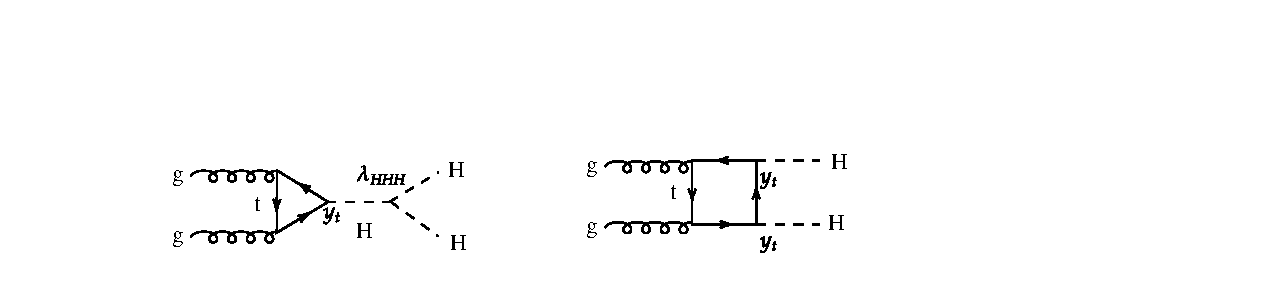
\includegraphics[width=1\linewidth]{Images/5.SPANet/gluon gluon fusion.pdf}
    \caption{Interfering Feynman diagrams showing di-Higgs production by gluon gluon fusion. The left (right) diagram is $\lambda$ dependent (independent).}
    \label{fig: GGF f}
\end{figure}

\begin{figure}[hbt]
    \centering
    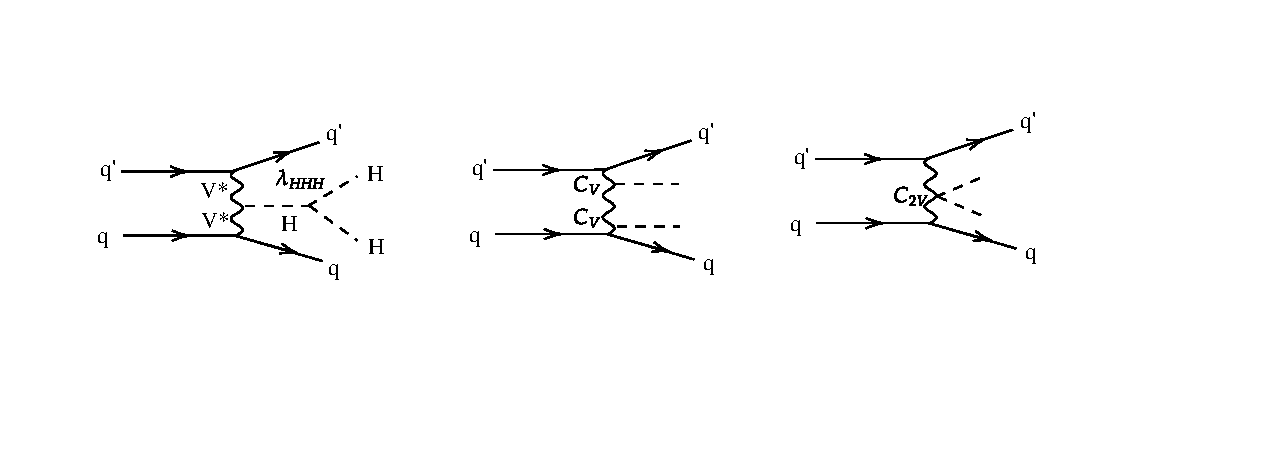
\includegraphics[width=1\linewidth]{Images/5.SPANet/VBF.pdf}
    \caption{Feynman diagram showing di-Higgs production by vector-boson fusion.}
    \label{fig: VF f}
\end{figure}

The branching ratios (BR) of the Higgs boson are shown in Figure \ref{fig: BR Higgs}. For $m_H=125$ GeV the highest BR is given by the $H\to b\Bar{b}$ channel. Proton-proton collisions occur at the LHC, therefore there is a high QCD background of multijet production, hence this channel has a low signal/background ratio (S/B). The analysis will focus on the HH $\to$ 4b decay channel in light of the very high BR in two b-quark pairs.

\begin{figure}[hbt]
    \centering
    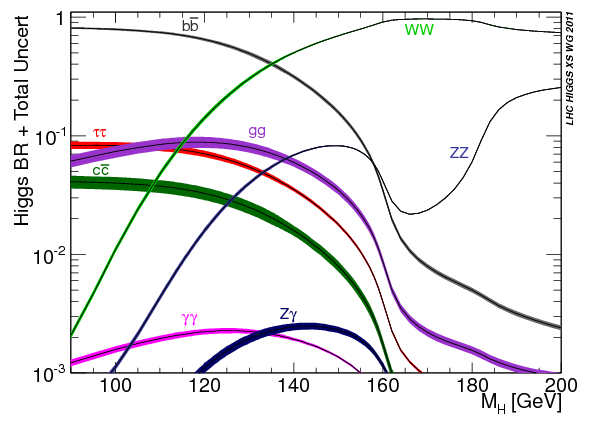
\includegraphics[width=0.7\linewidth]{Images/4.HH4b Analysis/Higgs intro/BR_higgs.png}
    \caption{Branching ratios and their uncertainties of the Higgs boson decay channels as a function of the Higgs mass $M_H$ \cite{BR_plot}.}
    \label{fig: BR Higgs}
\end{figure}

\noindent Two topologies arise from the decay of the double Higgs boson system \cite{talklucacometa}:
\begin{itemize}
    \item Resolved topology, where each $b$ quark is reconstructed as a separate jet with radius R=0.4
    \item Boosted topology, where the $H\to bb$ decay is reconstructed as a single large-radius jet with R=0.8 or 1
\end{itemize}

In the following Sections, the focus will be on the search for the HH $\to$ 4b in the ggF mode using the resolved topology.

\newpage

\subsubsection{Experimental signature of the HH $\to$ 4b topology} \label{subsection: topology}
Figure \ref{fig: topology} shows the topology of the HH $\to$ 4b decay. These 4b quarks in the final state will create a parton shower and hadronize into B hadrons and will be detected as jets in the detector. Therefore, the signature expected in the detector is represented by four small-radius b-jets (R=0.4) for the resolved topology.
\begin{figure}[hbt]
    \centering
    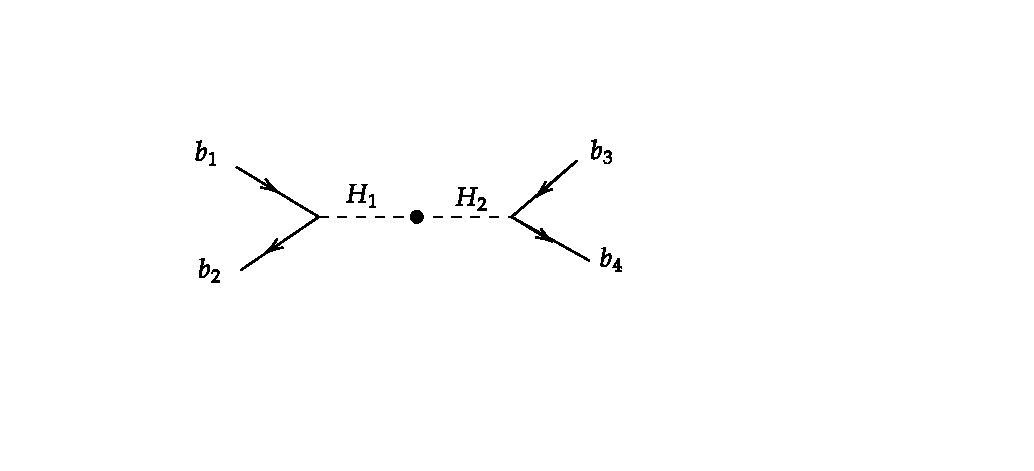
\includegraphics[width=0.5\linewidth]{Images/4.HH4b Analysis/Higgs intro/topology di-higgs.pdf}
    \caption{Topology of the $HH \to 4b$ decay.}
    \label{fig: topology}
\end{figure}

In the following, the so-called "leading Higgs" $H_1$ will correspond to the Higgs boson with the highest transverse momentum such that \pt($H_1$) > \pt($H_2$). $H_2$ will be referred to as the "subleading Higgs". The mass of the Higgs boson is 125 GeV, nevertheless, the mass of the reconstructed subleading Higgs tends to be slightly less ($\sim$ 120 GeV) mostly due to radiation leaking outside the cone of the b quark jet. 

\subsection{Results of the HH $\to$ 4b analysis in Run 2}

Figure \ref{fig: run 2 result kl} shows the results from the Run 2 analysis. The observed and expected 95\% confidence limits (CL) on the total cross section $\sigma_{ggF+VBF}$ HH as a function of \kl are shown. The total cross-section is defined as the sum of the ggF and VBF production modes. The observed (expected) upper limit at the 95 \% CL of the total cross-section is set to 3.9 (7.8) times the SM prediction. Moreover, the observed (expected) value of \kl is in the range -2.3 < \kl < 9.4 (-5.0 < \kl < 12.0 ) at the 95 \% CL. \cite{Run2res}

\begin{figure}
    \centering
    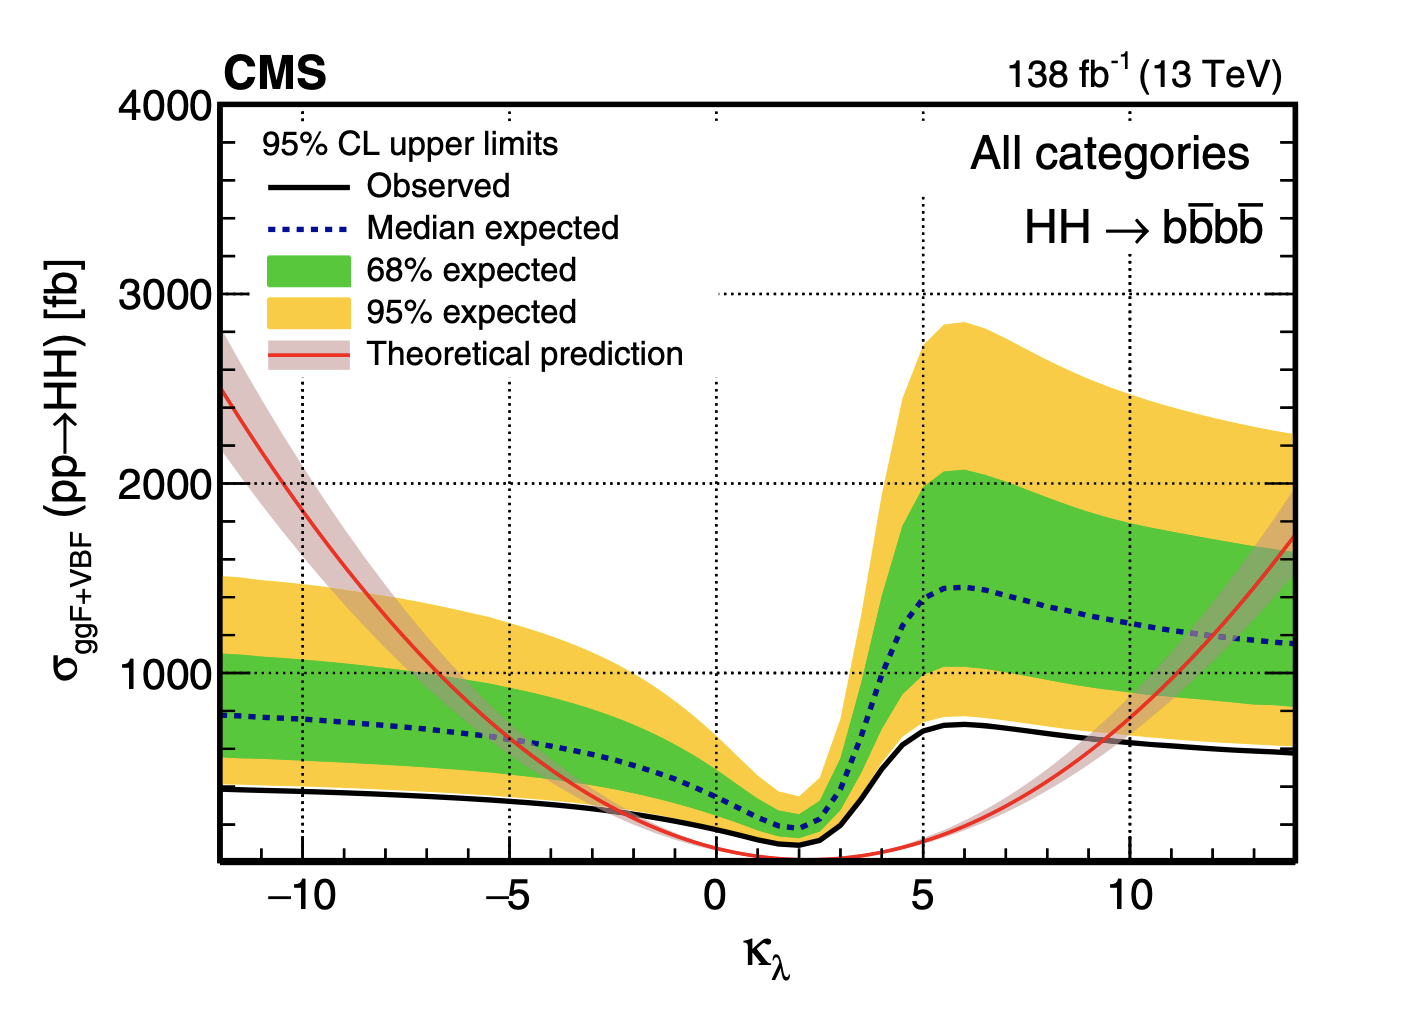
\includegraphics[width=0.7\linewidth]{Images/4.HH4b Analysis/DHH method/kl run 2 result.png}
    \caption{Observed and expected 95\% CL on the total cross-section $\sigma_{ggF+VBF}$ HH as a function of \kl. The green and yellow bands indicate the regions containing 68\% and 95\% of the limit values expected under the background-only hypothesis respectively. The theoretical cross-section expectation, assuming other couplings are set to the SM prediction, correspond to the red lines in this plot \cite{Run2res}.}
    \label{fig: run 2 result kl}
\end{figure}

\subsection{Simulations used in the HH $\to$ 4b search} \label{subsection: samples}

The results presented in Sections \ref{section: improving} and \ref{section: s/b classification} rely on Monte Carlo (MC) simulated events (for signal and QCD multijet) as well as proton-proton LHC Run 3 data collected in 2022. The signal events, i.e the HH production through the gluon-gluon fusion (ggHH) process are generated using \texttt{POWHEG} 2.0 \cite{Powheg} and interfaced with \texttt{PYTHIA} \cite{Pythia} for fragmentation and hadronization. The ggHH samples used in the following are:
\begin{itemize}
    \item SM CMS-official dataset, containing around 8M events with \kl=1
    \item \kl CMS-official dataset, containing around 100K events for \kl $\in \{0,2.45,5\}$
    \item \kl datasets generated with private productions, containing 1.5M events with $\kappa_\lambda 
\in \{-2.0, -1.0, 0.0, 0.5,$ $ 1.0, 1.5, 2.0, 2.45, 3.0, 3.5, 4.0, 5.0\} $
\end{itemize}

Although with the official datasets it is possible to use samples with \kl $\in \{0,1,2.45,5\}$, the private samples are used in Section \ref{subsection: kl} as they contain several more \kl simulated points compared to the CMS-official samples and have significantly more statistics. Figure \ref{fig: eta h1 for validation} shows a validation study performed to check the validity of the private samples by comparing the distribution of some observables to the distributions of the official datasets. Even though Figure \ref{fig: eta h1 for validation} only shows the pseudorapidity $\eta$ of the leading Higgs, the validation was also performed for the \pt, $\eta, m $ of the leading and subleading Higgs and the \pt, $\eta, m, \Delta \eta_{HH}, \Delta \Phi_{HH} $ of the di-Higgs system. Figure \ref{fig: eta h1 for validation} shows that the validation is successful, i.e. the privately-generated samples reproduce the kinematics of the official samples within the bin-by-bin statistical uncertainties of the samples.
\begin{figure}[h!]
    \centering
    \begin{subfigure}[b]{0.4\textwidth}
        \centering
        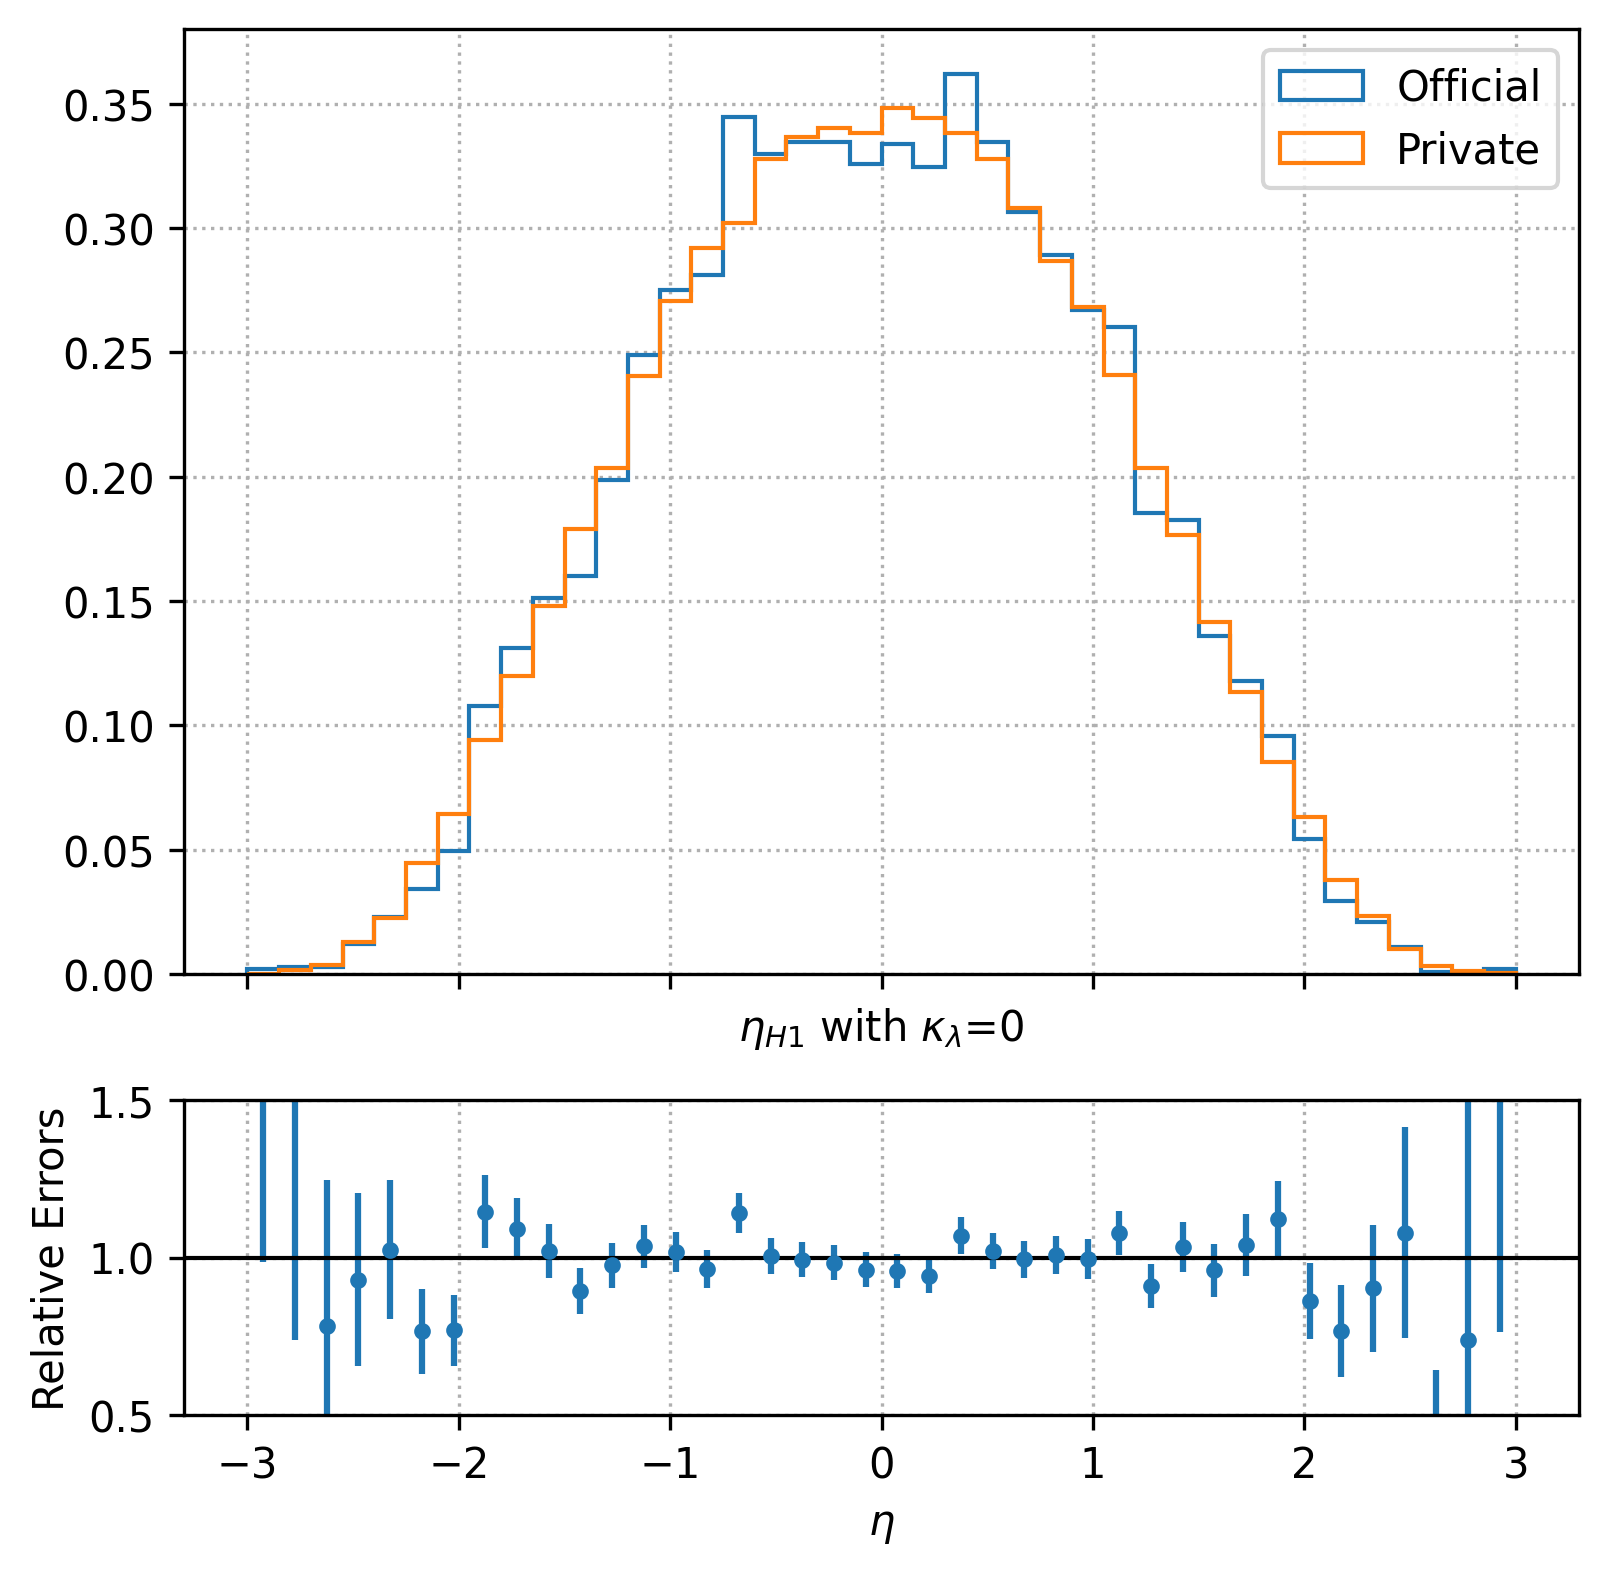
\includegraphics[width=\textwidth]{Images/4.HH4b Analysis/Validation plots/eta 0.png}
        % \caption{\kl=0}
        \label{fig: kl0}
    \end{subfigure}
    \hfill
    \begin{subfigure}[b]{0.4\textwidth}
        \centering
        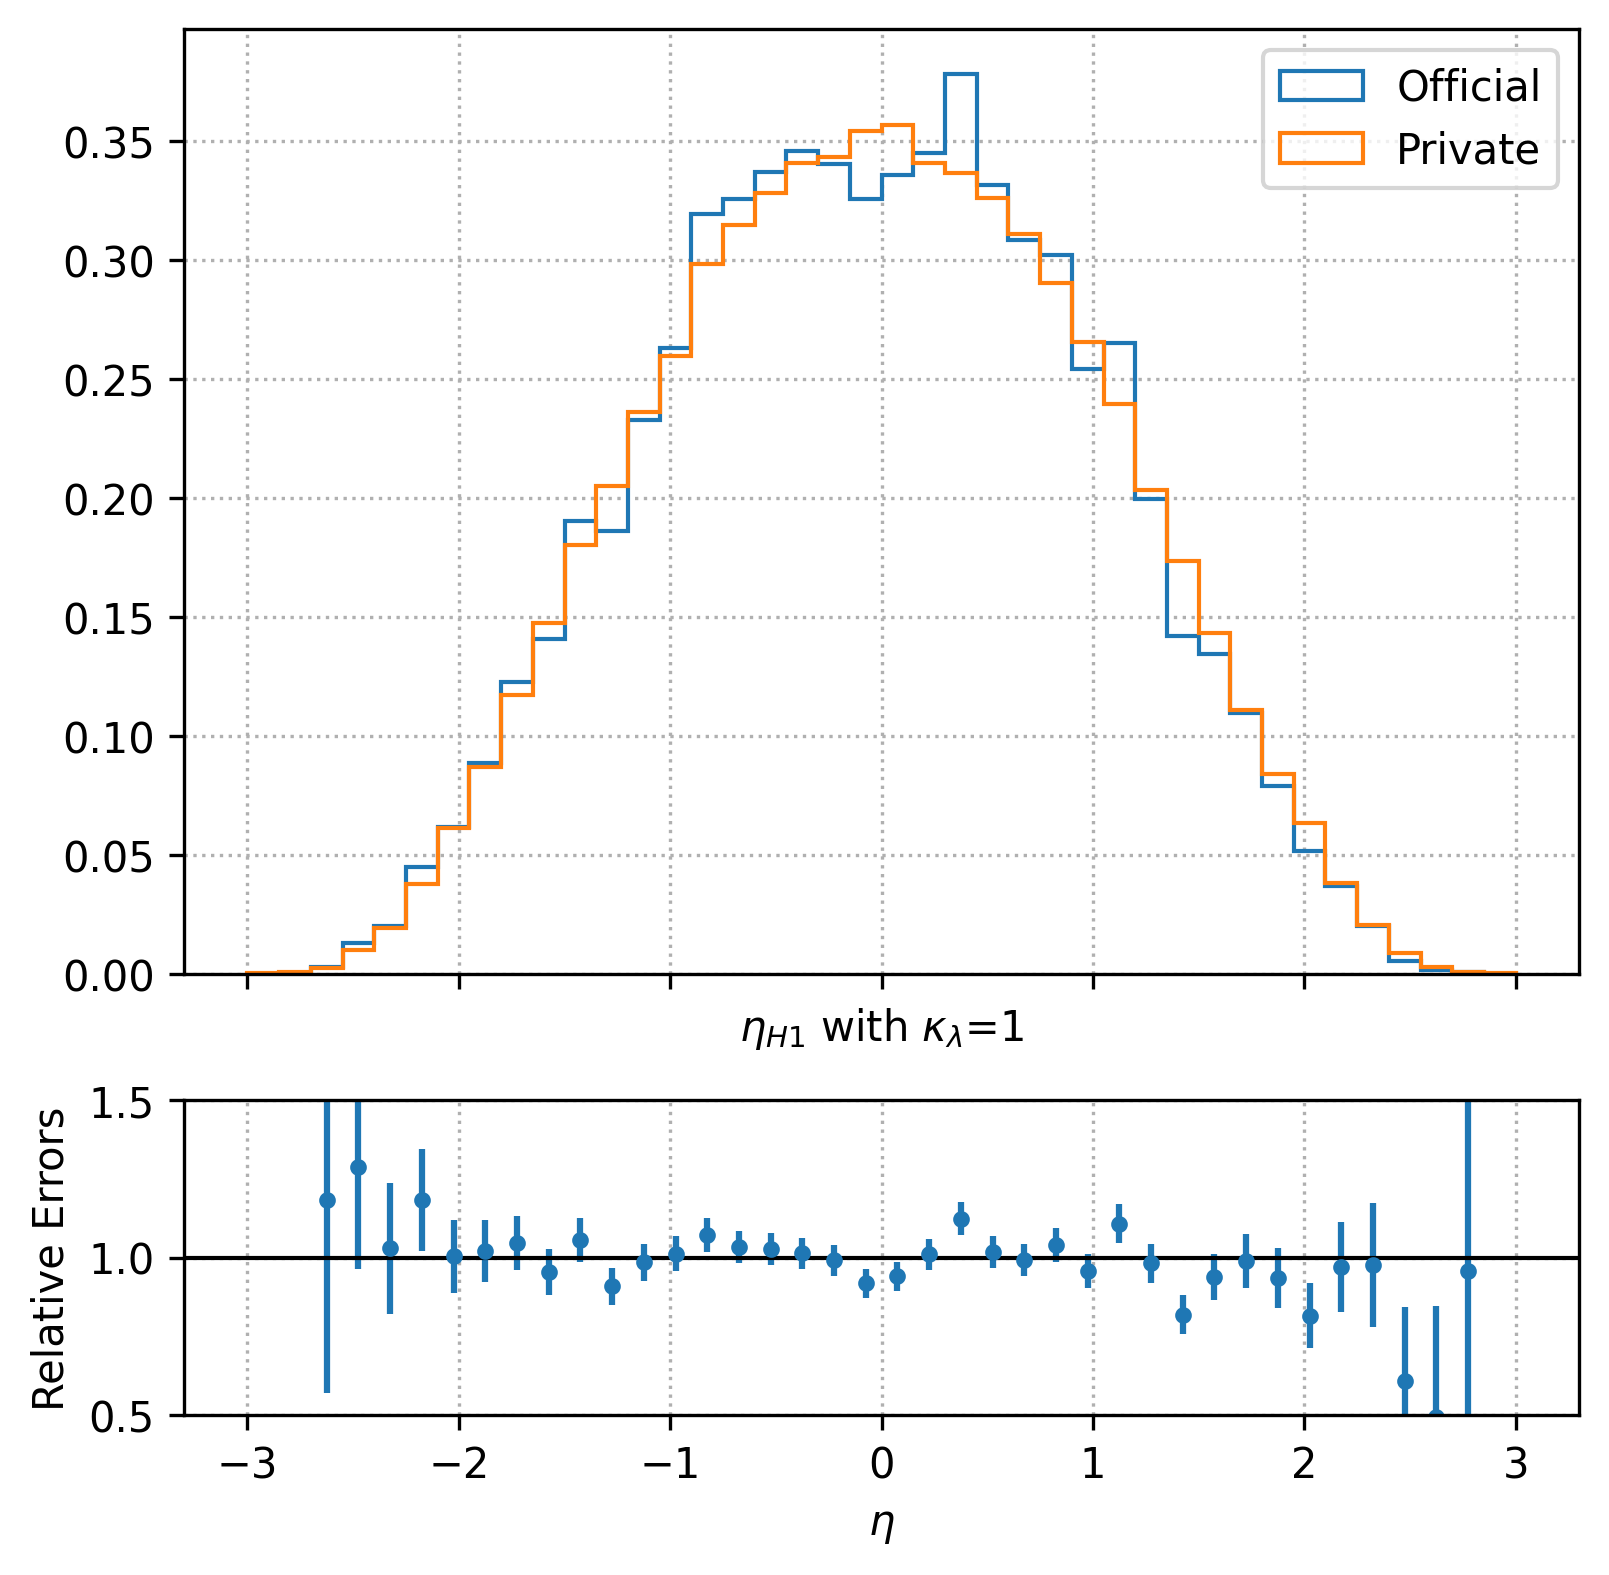
\includegraphics[width=\textwidth]{Images/4.HH4b Analysis/Validation plots/eta 1.png}
        % \caption{\kl=1}
        \label{fig: kl1}
    \end{subfigure}

    \vskip\baselineskip
    
    \begin{subfigure}[b]{0.4\textwidth}
        \centering
        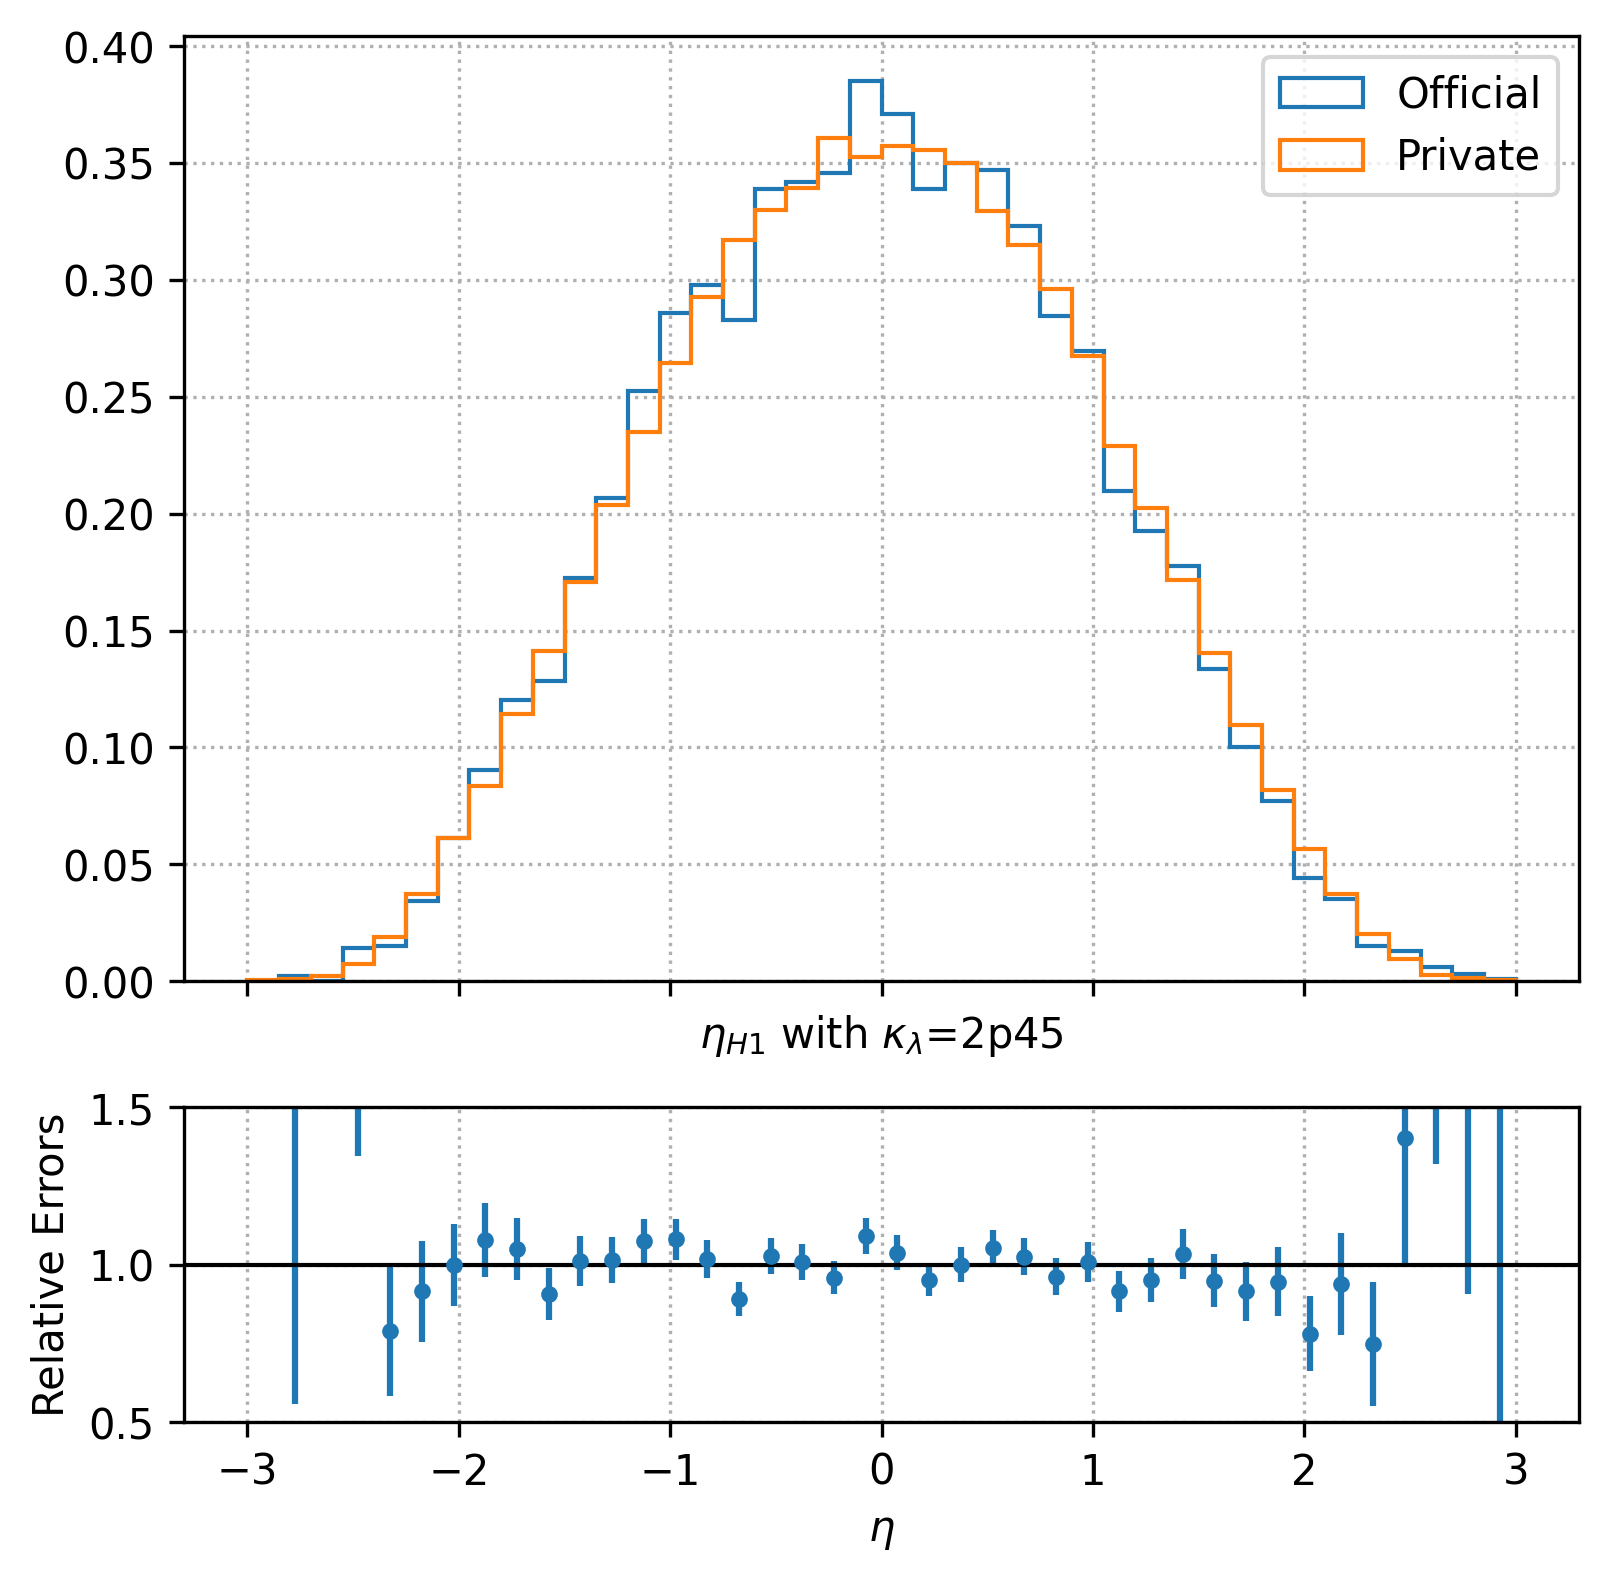
\includegraphics[width=\textwidth]{Images/4.HH4b Analysis/Validation plots/eta 2p45.png}
        % \caption{\kl=2.45}
        \label{fig: kl2p25}
    \end{subfigure}
    \hfill
    \begin{subfigure}[b]{0.4\textwidth}
        \centering
        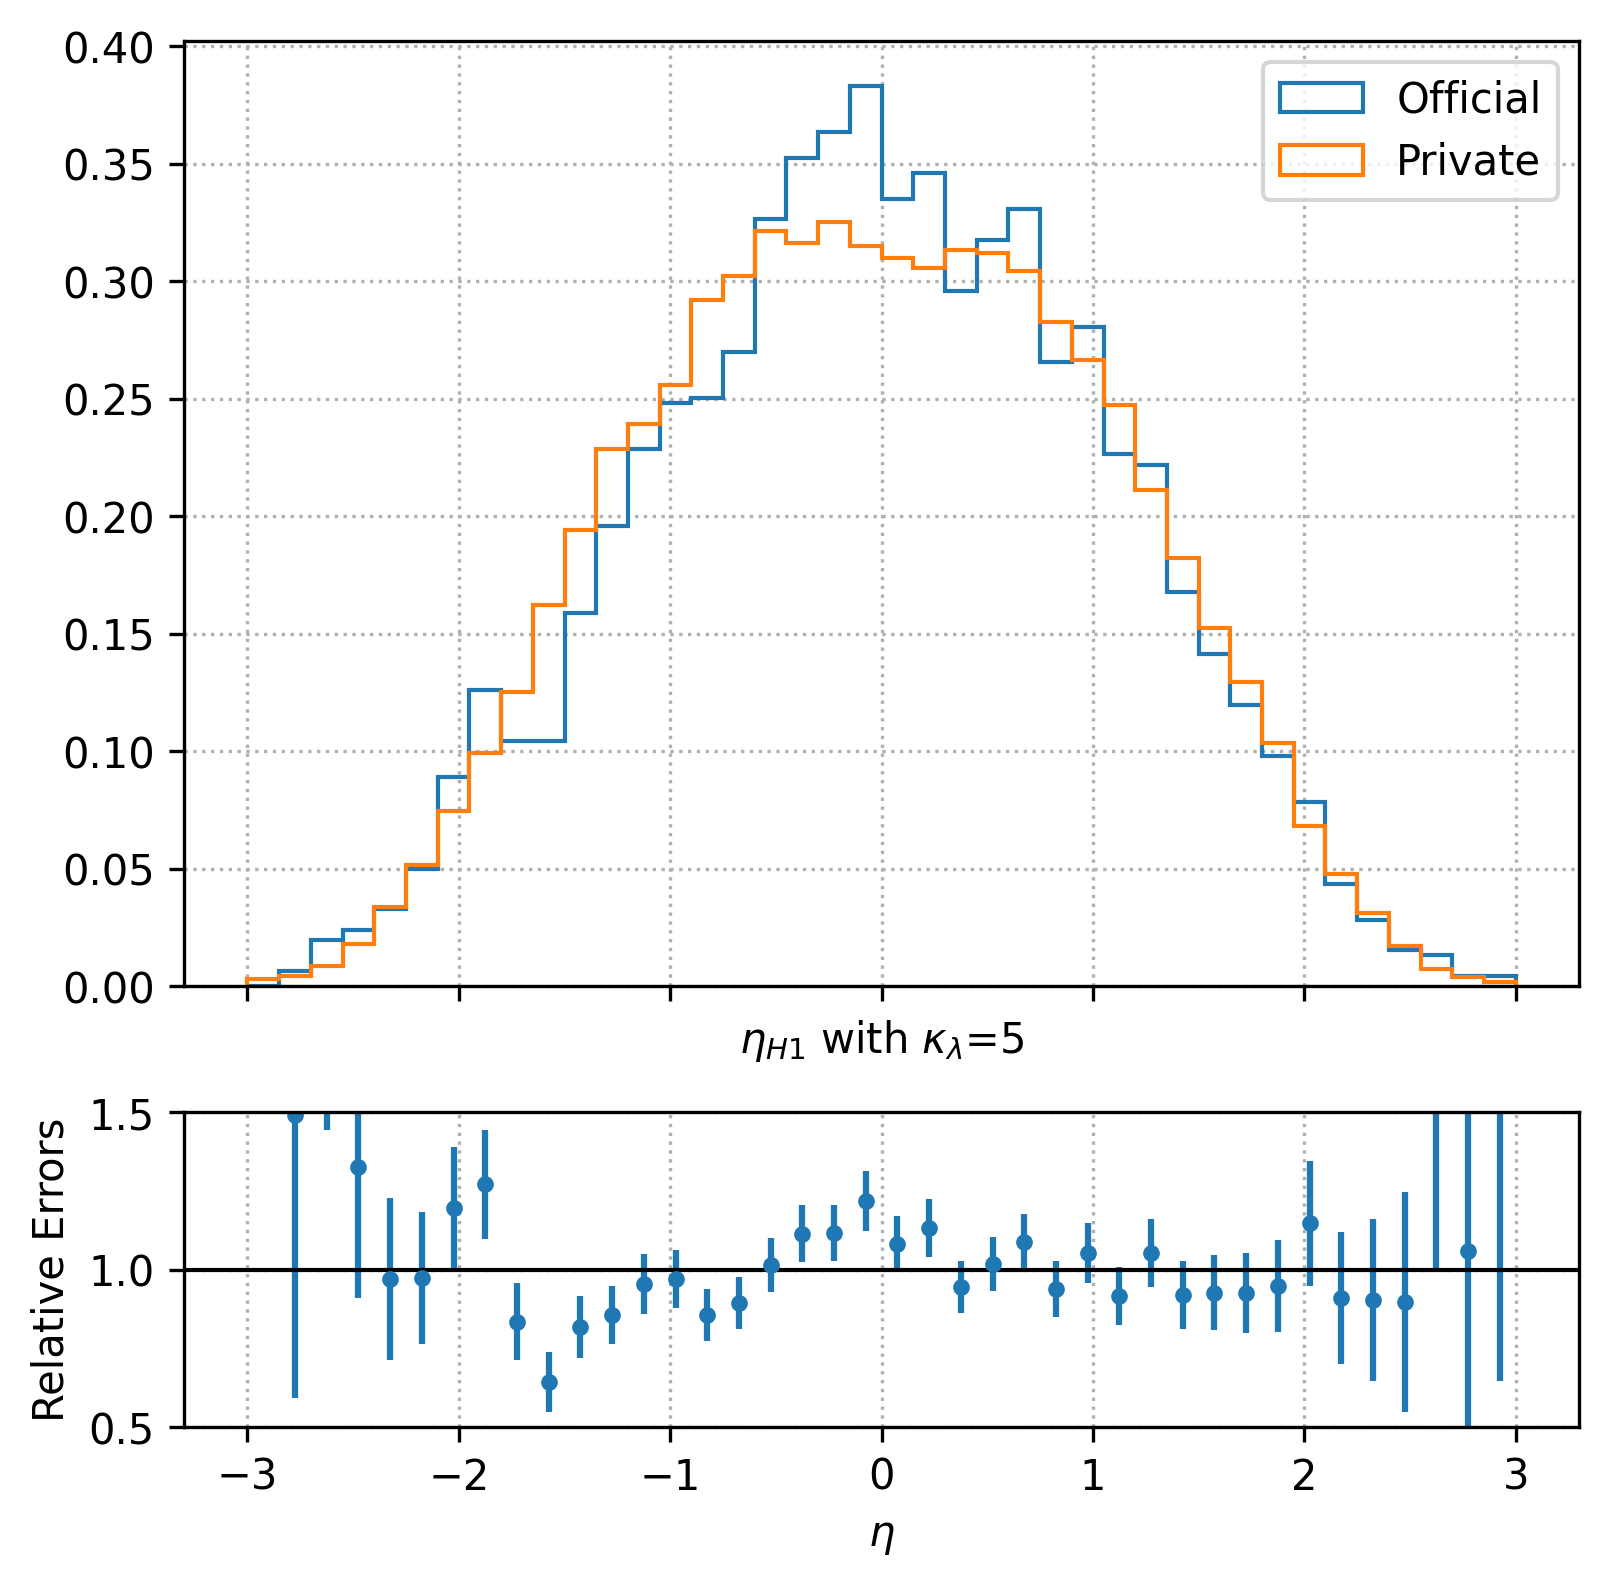
\includegraphics[width=\textwidth]{Images/4.HH4b Analysis/Validation plots/output.png}
        % \caption{\kl=5}
        \label{fig: kl5}
    \end{subfigure}
    
    \caption{Comparison of the pseudo-rapidity $\eta$ of the leading Higgs for different \kl values between the private and CMS-official signal samples.}
    \label{fig: eta h1 for validation}
\end{figure}

The main background HH $\to$ 4b analysis is represented by QCD multijet processes (Figure \ref{fig: QCD multijet}). This background is simulated using by \verb|MADGRAPH5_aMC@NLO| at leading order accuracy (LO) in the coupling constant $\alpha_s$ \cite{ANRun3}. The QCD multijet background is produced in \Ht bins, Table \ref{table: QCD  multijet} reports the different \Ht bins and the corresponding cross-sections \cite{ANRun3}.

\begin{figure}[hbt]
    \centering
    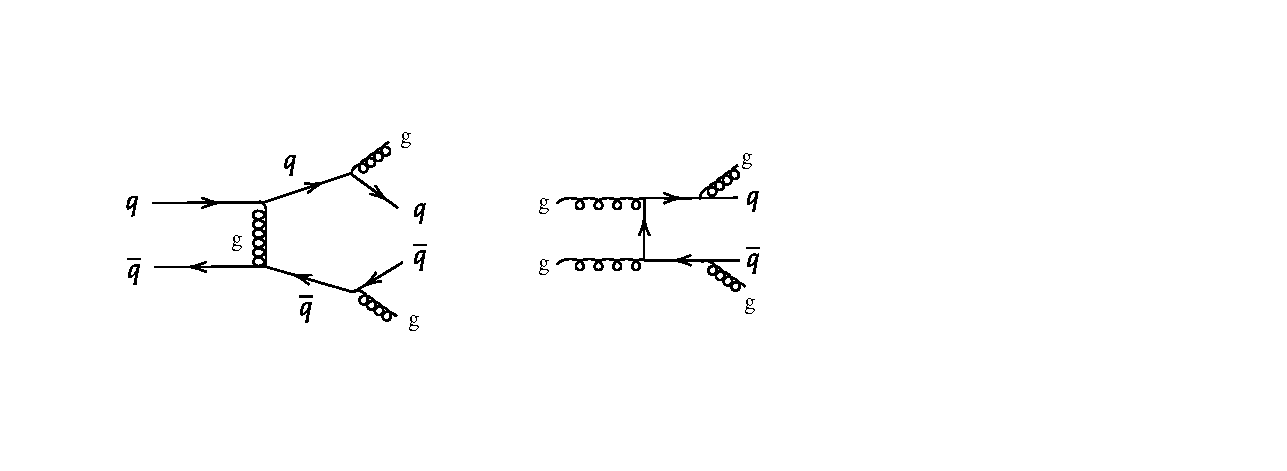
\includegraphics[width=0.6\linewidth]{Images/5.SPANet/QCD multijet.pdf} 
    \caption{Feynman diagram showing a QCD multijet process.}
    \label{fig: QCD multijet}
\end{figure}

\begin{table}[hbt]
    \centering
    \begin{tabular}{|c|c|}
        \hline
        \Ht bin [GeV] & $\sigma \times$ BR [pb] \\
       \hline
        200-400  & 1.968e+06 \\
        400 to 600  &  1.000e+05\\
        600 to 800 & 1.337e+04 \\
        800 to 1000 &  3.191e+03\\
        1000 to 1200  &  8.997e+02\\
        1200 to 1500 & 3.695e+02 \\
        1500 to 2000  & 1.272e+02 \\
        from 2000 on  & 2.514e+01 \\
    \hline
    \end{tabular}
    \caption{List of \Ht bins produced for the QCD MC multijet background with their corresponding cross-sections.}
    \label{table: QCD  multijet}
\end{table}

Data samples are used to test the background mass sculpting in Section \ref{subsection: bckg mass sculpting} and as background for the classification in Section \ref{section: s/b classification}. These datasets contain data collected by CMS in proton-proton collisions in Run 2022 E, during Run 3. The dominant process is QCD multijet. Therefore, in the following, the background will always refer to the QCD multijet process. Nevertheless, a distinction will be made between MC-produced QCD samples (QCD MC) and data QCD samples (data) from Run 3.

\newpage

\subsection{Analysis kinematic selection} \label{subsection:cutflows}

This Section reports the characteristics of the kinematic selections employed in the analysis, with dedicated focus on the set of Tight cuts used in the analysis and the Loose cuts that are applied to the Run 3 data.

\begin{table}[hbt]
\centering
\begin{tabular}{|M{3cm}||M{12cm}|}
 \hline
 HLT  & \begin{verbatim}
    QuadPFJet70_50_40_35_PFBTagParticleNet_2BTagSum0p65
\end{verbatim} \\
 \hline
 Lepton Veto & \begin{itemize}
     \item e ($\mu$): \pt >15 (10) GeV,  $\eta$<2.4 
     \item e ($\mu$): \verb|mvaIso_WP80| (looseID)
     
     \item PF Iso $(\Delta R < 0.3) < 0.15$
     
     \item $d_{xy}$ barrel <0.05
     \item $d_{z}$ barrel <0.1
     \item $d_{xy}$ endcap <0.1
     \item $d_{z}$ endcap <0.2
 \end{itemize} \\
 \hline
 $\geq$ 4b jet candidates & \begin{itemize}
     \item \pt > 35 GeV
     \item $\eta$ < 2.5
     \item jetID with Lepton Veto
 \end{itemize} \\
 \hline
 HH reconstruction & \begin{itemize}
     \item 4 jets with Highest PNet b-tag score
     \item Jets ordered in \pt:
            \begin{itemize}
                \item \pt > [80,60,45,35]
            \end{itemize}
     \item Jets ordered in b-tag:
        \begin{itemize}
            \item Mean PNet of the leading 2 b-tag jets > 0.65
            \item 3° and 4° jet PNet b-tag > 0.2605 
        \end{itemize}
 \end{itemize}\\
 \hline
\end{tabular}
\caption{Tight cuts applied to the samples used in Sections \ref{section: improving} and \ref{section: s/b classification}. The trigger (HLT defined in Section \ref{section: CMS}) requirement is shown: 4 jets with \pt > [70,50,40,35] and the mean of the b-tag score of 2 of the jets to be above 0.65. Additionally, kinematic requirements of the four or more b jets required for the analysis are shown. Finally, the method to reconstruct the HH is reported.}
\label{table: Tight cuts}
\end{table}

\begin{table}[hbt]
\centering
\begin{tabular}{|M{3cm}||M{12cm}|}
 \hline
 HLT  & 
 \begin{verbatim}
    QuadPFJet70_50_40_35_PFBTagParticleNet_2BTagSum0p65
\end{verbatim}\\
 \hline
 Lepton Veto & \begin{itemize}
     \item e ($\mu$): \pt >15 (10) GeV,  $\eta$<2.4 
     \item e ($\mu$): \verb|mvaIso_WP80| (looseID)
     \item PF Iso $(\Delta R < 0.3) < 0.15$
     \item $d_{xy}$ barrel <0.05
     \item $d_{z}$ barrel <0.1
     \item $d_{xy}$ endcap <0.1
     \item $d_{z}$ endcap <0.2
 \end{itemize} \\
 \hline
 $\geq$ 4b jet candidates & \begin{itemize}
     \item \pt > 25 GeV
     \item $\eta$ < 2.5
     \item jetID with Lepton Veto
 \end{itemize} \\
 \hline
 HH reconstruction & \begin{itemize}
     \item All jets passing the preselections
     \item Jets ordered in \pt:
            \begin{itemize}
                \item \pt > [80,60,45,35]
            \end{itemize}
     \item Jets ordered in b-tag:
        \begin{itemize}
            \item Mean PNet of the leading 2 b-tag jets > 0.65
            \item 3° and 4° jet PNet b-tag > 0.2605 
        \end{itemize}
 \end{itemize}\\
 \hline
\end{tabular}
\caption{Loose cuts applied to the Run 3 data. The trigger (HLT defined in Section \ref{section: CMS}) is shown, which requires 4 jets with \pt > [70,50,40,35] and the mean of the b-tag score of 2 of the jets to be above 0.65. Additionally, kinematic requirements of the four or more b jets required for the analysis are shown. Finally, the method to reconstruct the HH is reported.}
\label{table: Loose cuts}
\end{table}

Tables \ref{table: Tight cuts} and \ref{table: Loose cuts} outline the HLT selection and Lepton veto requirements when applying the Tight or Loose cuts respectively. They also report the preselections of the four or more jets considered for the analysis as well as the HH reconstruction requirements.  When applying Loose cuts, the jets are required to have a \pt > 25 GeV while for the Tight cuts the requirement is \pt > 35 GeV. Moreover, when applying the Tight cuts for the HH reconstruction only the 4 jets with the highest PNet b-tag score are considered whereas in the Loose cuts all the jets passing the preselections specified in Table \ref{table: Loose cuts} are considered. 

Applying the Tight cuts to the official SM signal sample (with \kl=1), containing around 8M events before preselections, results in a reduction to 1.7M events while applying Loose cuts to this sample results in a reduction to 2.1M events. This leads to an increase of 24\% in the number of events. Figure \ref{fig: validation cuts} shows the comparison of the distributions for the \pt and the invariant mass of the leading and sub-leading Higgs boson for \kl=1 when applying Loose and Tight cuts. This study was performed for different values of \kl but only \kl=1 is shown. The distribution of the newly added events when considering Loose cuts, i.e. the events where at least one of the jets in the event has \pt $\in [25-35]$ GeV, is also shown. It is to note that when applying the Loose cuts the \pt and invariant mass distributions are shifted to the left. This feature is studied by looking at the distribution of the newly added events, which have lower \pt and therefore shift the total distribution towards lower \pt and mass.

Table \ref{table: SE kl 1} shows the signal efficiency for \kl=\{1,0,2.45,5\}. As expected, the signal efficiency is higher when the Loose cuts are applied.

\begin{figure}[h!]
    \centering
    \begin{subfigure}[b]{0.4\textwidth}
        \centering
        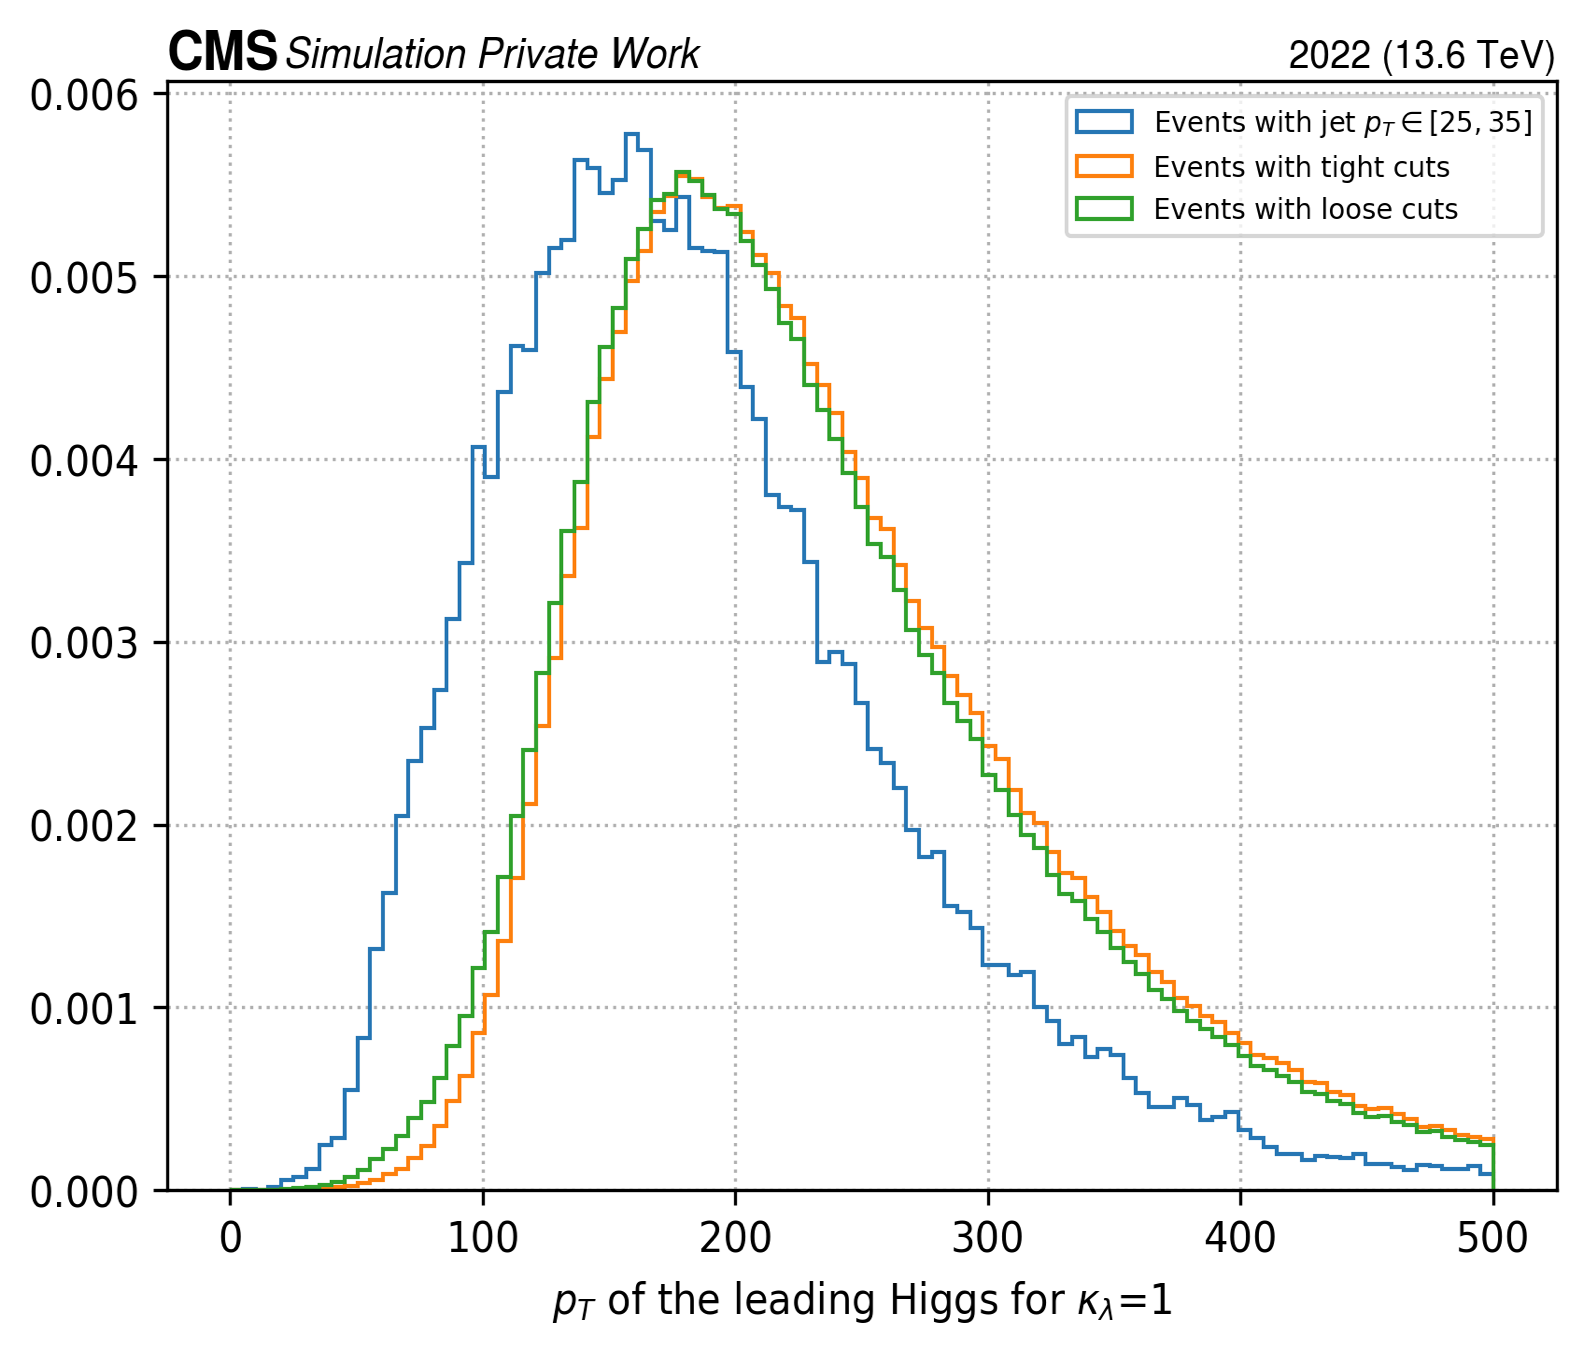
\includegraphics[width=\textwidth]{Images/4.HH4b Analysis/New events/pt h1.png}
        % \caption{\pt of the leading Higgs.}
        \label{fig: pt h1}
    \end{subfigure}
    \hfill
    \begin{subfigure}[b]{0.4\textwidth}
        \centering
        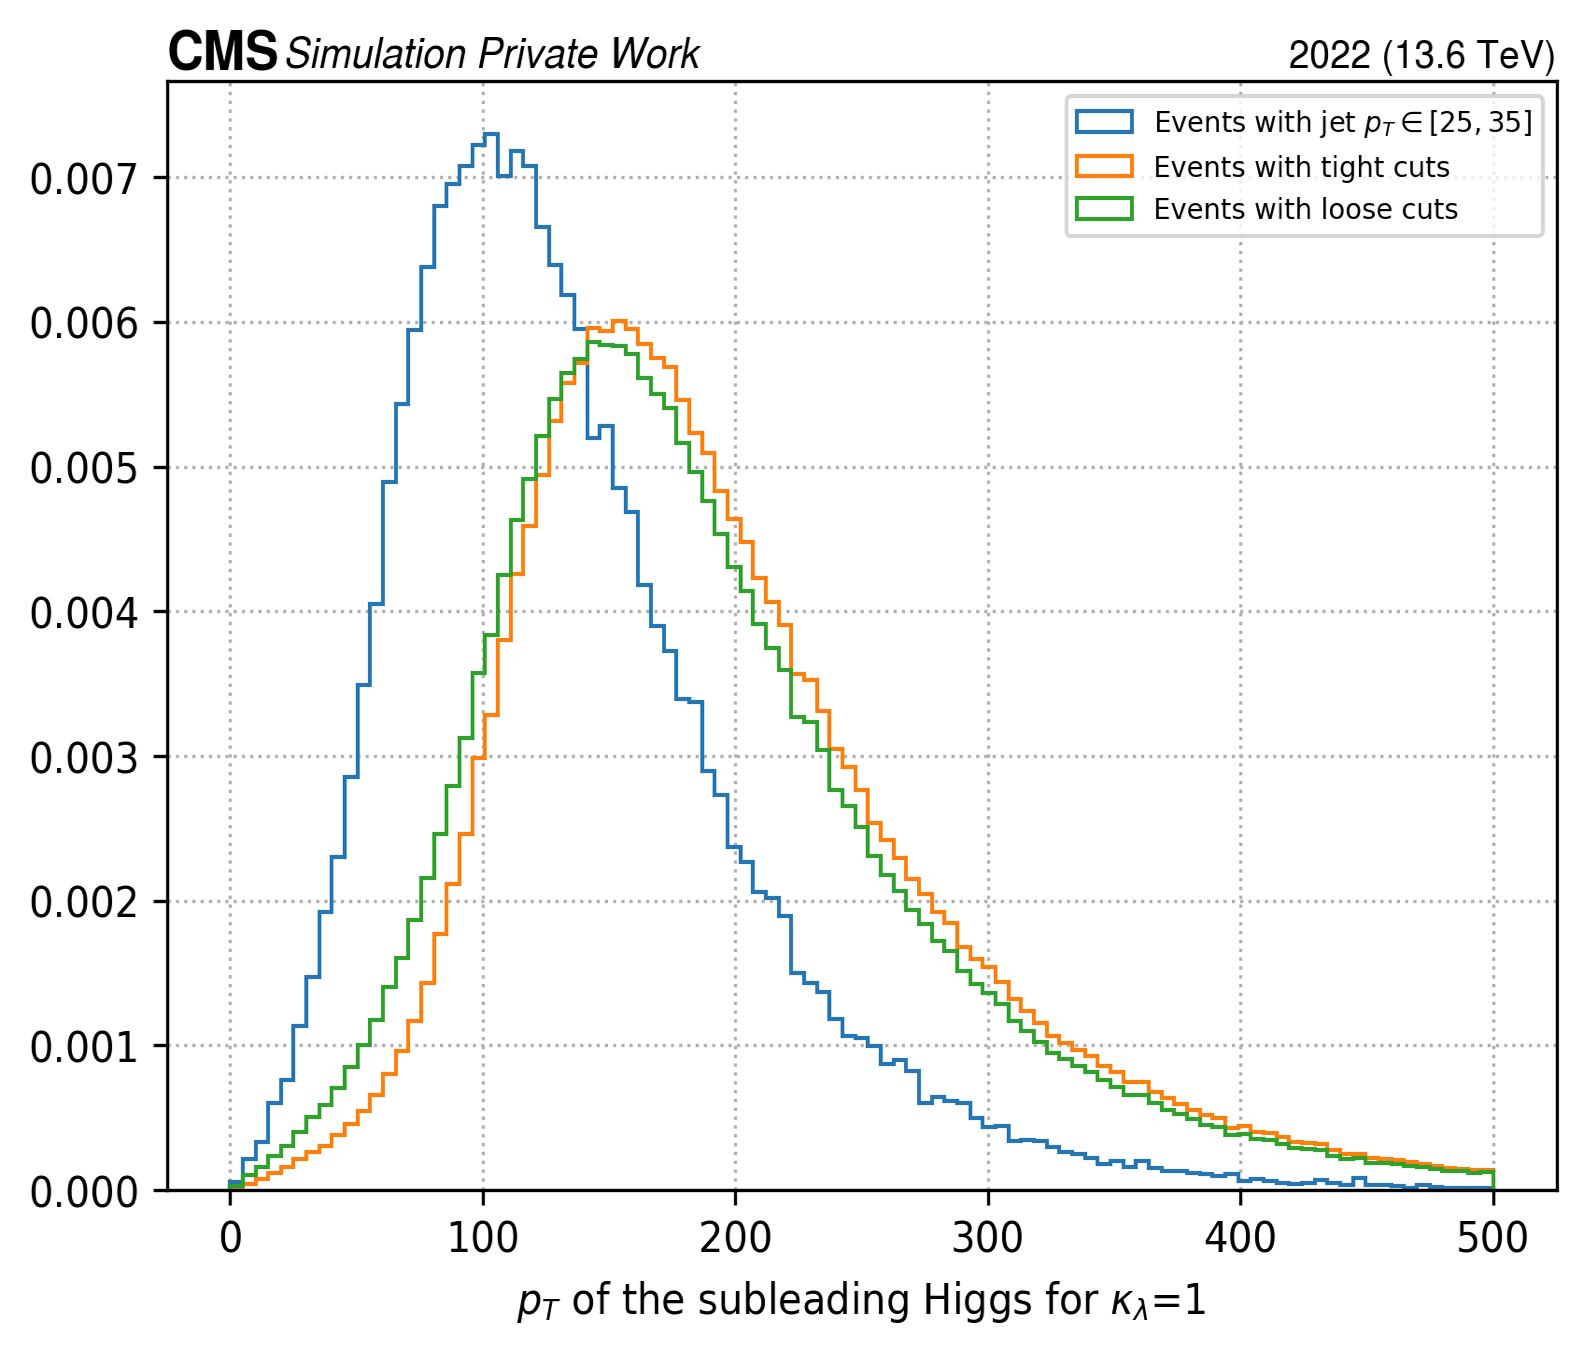
\includegraphics[width=\textwidth]{Images/4.HH4b Analysis/New events/pt h2.png}
        % \caption{\pt of the subleading Higgs.}
        \label{fig: pt h2}
    \end{subfigure}

    \vskip\baselineskip
    
    \begin{subfigure}[b]{0.4\textwidth}
        \centering
        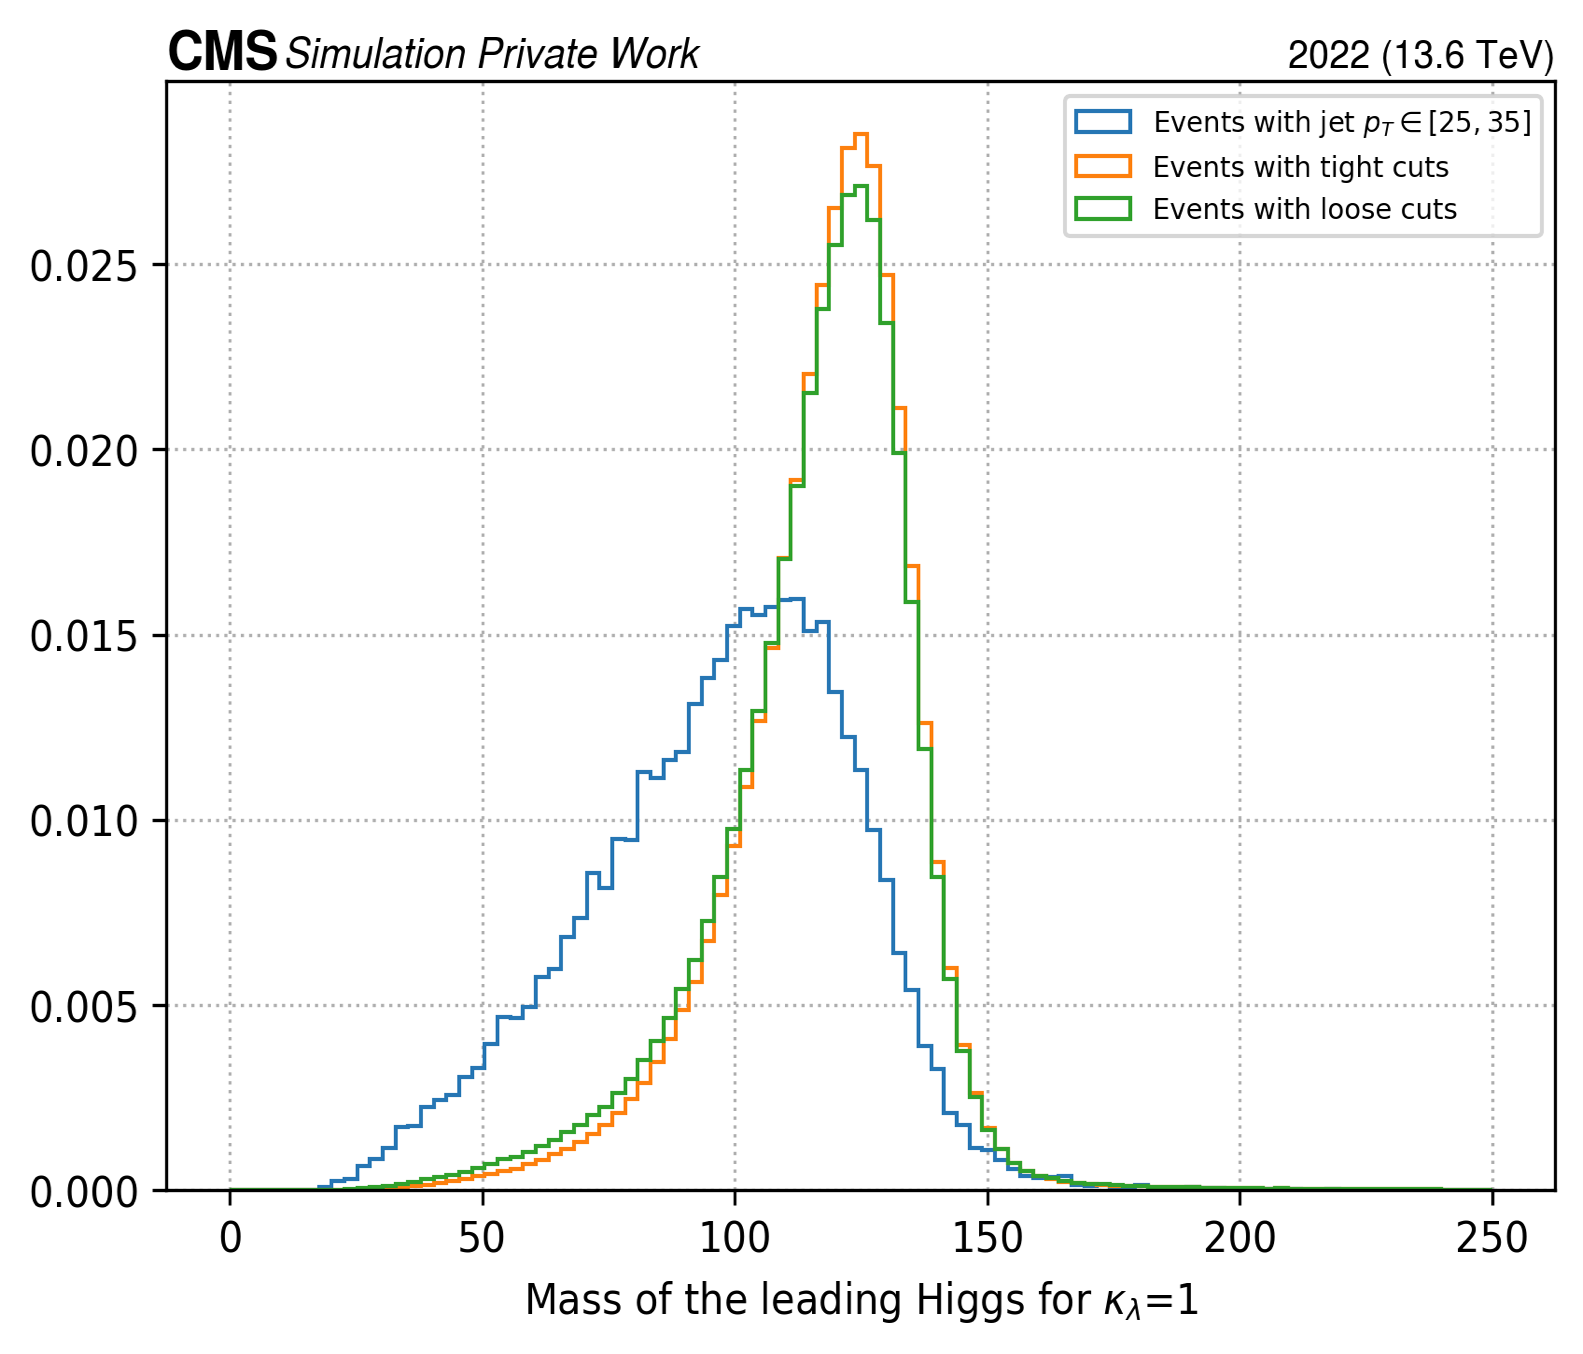
\includegraphics[width=\textwidth]{Images/4.HH4b Analysis/New events/mass h1.png}
        % \caption{Invariant mass of the leading Higgs.}
        \label{fig: m h1}
    \end{subfigure}
    \hfill
    \begin{subfigure}[b]{0.4\textwidth}
        \centering
        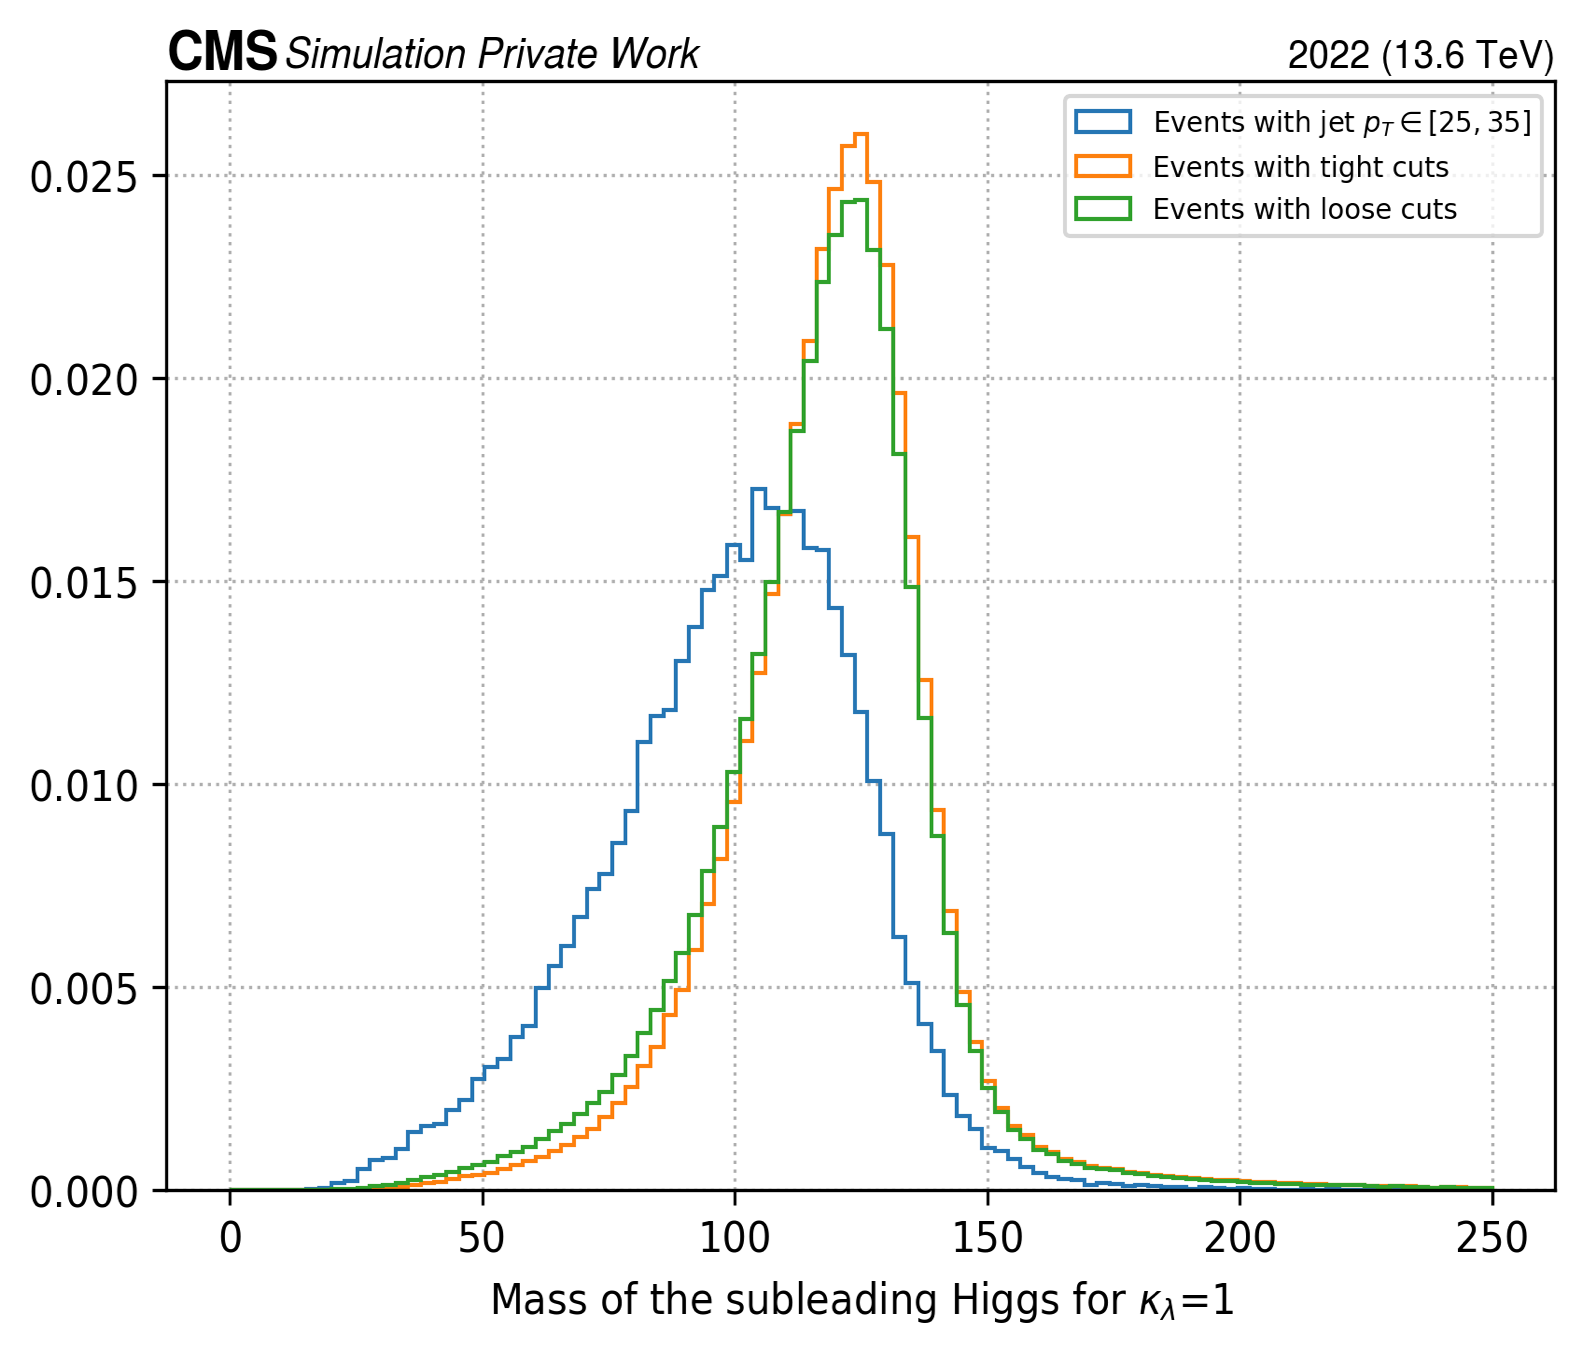
\includegraphics[width=\textwidth]{Images/4.HH4b Analysis/New events/mass h2.png}
        % \caption{Invariant mass of the subleading Higgs.}
        \label{fig: m h2}
    \end{subfigure}
    
    \caption{Comparison of the distribution of two different observables \pt and mass of the leading and the subleading Higgs when Tight and Loose cuts are applied. The newly added events by the Loose cuts are also shown in these plots.}
    \label{fig: validation cuts}
\end{figure}

\clearpage

\begin{table}[hbt]
\centering
    \begin{tabular}{ |p{10cm}|p{3cm}| }
 \hline
 \multicolumn{2}{|c|}{$\kappa_\lambda$=1} \\
 \hline
 Initial number of events & 7 391 383 \\
 Signal efficiency in the 4b region with the {Tight cuts}  & 8.77 \%\\
 Signal efficiency in the 4b region with the {Loose cuts}  &  10.51 \% \\
 \hline
 \multicolumn{2}{|c|}{Private sample for $\kappa_\lambda$=0} \\
 \hline
 Initial number of events & 1 494 015 \\
 Signal efficiency in the 4b region with the Tight cuts  & 6.95 \% \\
 Signal efficiency in the 4b region with the Loose cuts  &  8.57 \% \\
 \hline
 \multicolumn{2}{|c|}{Private sample for $\kappa_\lambda$=2.45} \\
 \hline
 Initial number of events & 1 489 001 \\
 Signal efficiency in the 4b region with the Tight cuts  & 9.17 \% \\
 Signal efficiency in the 4b region with the Loose cuts  &  10.92 \% \\
 \hline
         \multicolumn{2}{|c|}{Private sample for $\kappa_\lambda$=5} \\
         \hline
         Initial number of events & 1 496 012 \\
         Signal efficiency in the 4b region with the Tight cuts  & 2.81 \% \\
         Signal efficiency in the 4b region with the Loose cuts  &  4.12 \% \\
         \hline
 \end{tabular}
\caption{Comparison of the signal efficiency when applying Loose or Tight cuts to the CMS-official sample for different \kl values}
\label{table: SE kl 1}
\end{table}

\clearpage

\subsection{Definition of analysis regions based on b-tag requirements} \label{subsubsecxtion: 4/2 b regions}

Based on the multiplicity of the b-tagged jets, the datasets are classified into two regions. 

\vspace{0.2 cm}

\noindent The 2b region requires:
\begin{itemize}
    \item Mean PNet of the leading 2 b-tag jets > 0.65
    \item Veto on the 3° and 4° jet PNet b-tag < 0.2605
\end{itemize}

\vspace{0.2 cm}

\noindent The 4b region requires:
\begin{itemize}
    \item Mean PNet of the leading 2 b-tag jets > 0.65
    \item 3° and 4° jet PNet b-tag > 0.2605
\end{itemize}

\vspace{0.2 cm}

\noindent It is possible to define 2b data (QCD) as the data (QCD) sample in which the requirements of the 2b region are applied and 4b data (QCD) as the data (QCD) sample in which the requirements of the 4b region are applied.

\subsection{Signal and control regions}

The signal region (SR)  has a large S/B ratio. The control region (CR), has a low S/B that is kinematically similar to the SR to ensure the validity of the background prediction extrapolation from CR to SR.  Control regions are used to extract the background model (shape and normalisation of the background processes) and extrapolate it to the SR. For this analysis, a radial distance from (125,120) GeV in the $m_{H1}-m_{H2}$ is defined as follows \cite{ANRun2}:
\begin{equation}
    R_{HH}(m_{H1}, m_{H2})=\sqrt{(m_{H1}-125)^2+(m_{H2}-120)^2}
\end{equation}
The SR is defined such that $R_{HH} < 30$ GeV and the CR such that $30 < R_{HH} < 55$ GeV.

\begin{figure}
    \centering
    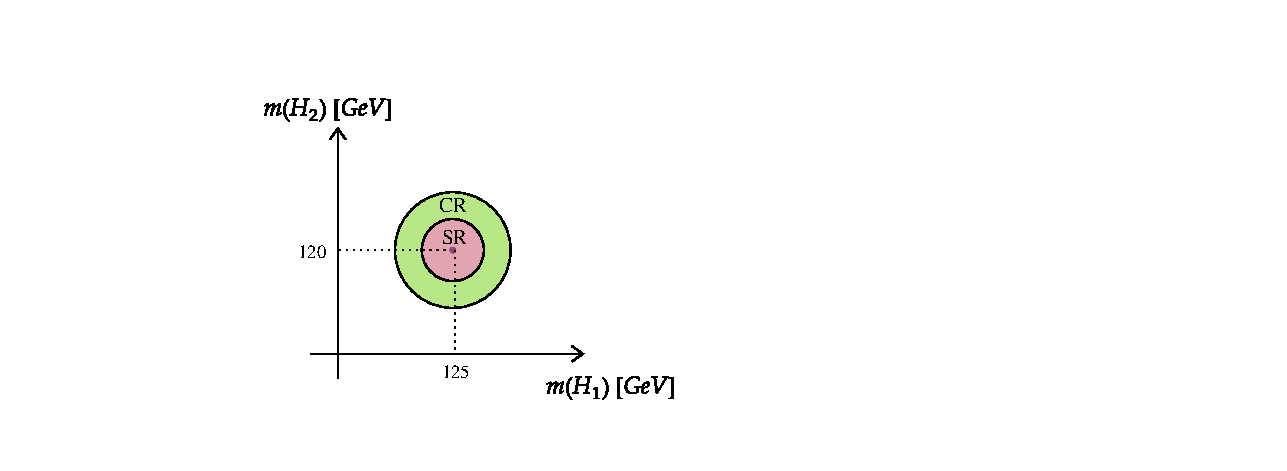
\includegraphics[width=0.7\linewidth]{Images/4.HH4b Analysis/Higgs intro/CR - SR.pdf}
    \caption{Sketch of the signal and control regions in the $m_{H1}$ and $m_{H2}$ plane.}
    \label{fig:enter-label}
\end{figure}

\subsubsection{Background estimation} \label{subsection: bckg estimation}

To estimate the background, a data-driven approach is used in this analysis due to the inadequate modeling of the QCD-induced multijet processes. This approach uses a multidimensional kinematic reweighting technique. In this case, the 2b data observables are reweighted to match the distributions of the 4b data observables. To do so, a neural network is trained to separate data events in the CR of the 2b region (CR$_{\text{2b}}$) from the data events in the CR of the 4b region (CR$_{\text{4b}}$). The outcome of this network is the transfer function which gives the reweighting factor applied to CR$_{\text{2b}}$ data to match the distributions in the  CR$_{\text{4b}}$ region both in shape and normalisation. The 2b data to which we have applied these reweighting factors is the so-called "4b-morphed data".


\subsection{Algorithm for jet pairing used in Run 2 HH $\to$ 4b analysis} \label{subsection: run2 pairing}

At least 4 jets coming from a signal event are reconstructed in the presence of the HH $\to$ 4b signal. To identify this event as a signal event, 4 of the reconstructed jets have to be matched to the corresponding generator-level quarks. It is important to note that there are two internal symmetries for this pairing: one regarding the exchange of the number of the jet paired to the generator-level $b$ quark coming from the Higgs, as the reconstruction cannot distinguish between quark and anti-quark; and another one regarding the exchange of the Higgs candidates. As long as the jets are correctly paired, it is not important whether they come from $H_1$ or $H_2$. Taking these symmetries into account, when considering 4 jets for the pairing (0,1,2,3), there are 3 possible combinations for the pairing, given by A, B, and C.

\begin{equation*}
   \text{Combination A}:[(0,1),(2,3)] 
\end{equation*}
\begin{equation*}
   \text{Combination B}:[(0,2),(1,3)] 
\end{equation*}
\begin{equation*}
   \text{Combination C}:[(0,3),(1,2)] 
\end{equation*}

In the HH $\to$ 4b Run 2 analysis, the so-called "$D_{HH}$-method" is used for the pairing. To define the goodness of the pairing with this method a distance to the diagonal in the $m_{H1}-m_{H2}$ plane is defined, sketched in Figure \ref{fig: diagonal method} \cite{ANRun2}:

\begin{equation}
    D_{HH}=\frac{|M_{H_1}- \kappa M_{H_2}|}{\sqrt{1+\kappa^2}}
    \label{eq: dist dhh}
\end{equation}
\noindent with $\kappa=\frac{m_{H1}}{m_{H2}}=\frac{125}{120}=1.04$, accounting for the difference between the two reconstructed Higgs masses. If the pairing is correct, it is expected that $D_{HH}$ is closer to the diagonal as shown in Figure \ref{fig: diagonal method}. This distance is computed for all the possible combinations, namely $D_{HH}^A$, $D_{HH}^B$, and $D_{HH}^C$. The algorithm aiming at choosing the most successful pairing among the possible combinations works as follows:
\begin{itemize}
    \item The $D_{HH}$ distances are ordered from smallest to highest: $D^1_{HH}$ < $D^2_{HH}$ < $D^3_{HH}$
    \item The difference $\Delta D_{HH}= |D_{HH}^1- D_{HH}^2|$ between the two smallest distances is computed.
        \begin{itemize}
            \item If $\Delta D_{HH} > 30$ GeV the pairing used is the one given by the combination corresponding to $D_{HH}^1$, the latter being the smallest distance.
            \item If $\Delta D_{HH} < 30$ GeV it is not possible to select the smallest distance as previously described due to the resolution of the mass distributions. Therefore, the distance (either $D_{HH}^1$ or $D_{HH}^2$) having the Higgs with the largest \pt at the center of mass frame (\pt$(H)^*$) is chosen.
        \end{itemize}
\end{itemize}

\begin{figure}
    \centering
    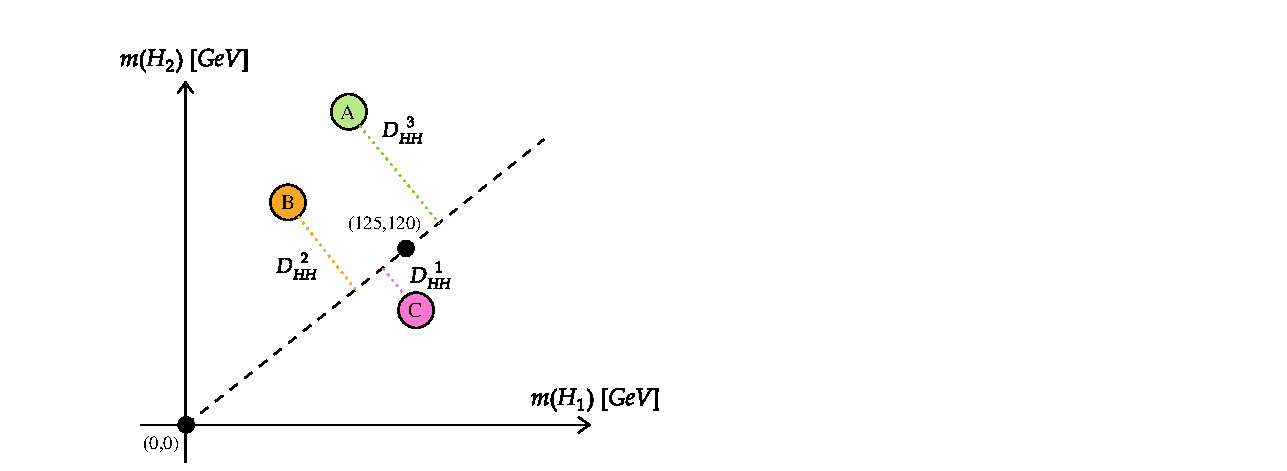
\includegraphics[width=0.7\linewidth]{Images/4.HH4b Analysis/DHH method/Dhh method.pdf}
    \caption{Sketch of the "$D_{HH}$-method" that uses the distance to the diagonal line in the mass plane to determine the best pairing of jets to reconstruct $H_1$ and $H_2$.}
    \label{fig: diagonal method}
\end{figure}


As an alternative to the $D_{HH}$-method for jet pairing, SPANet (discussed in Section \ref{section: spanet architecture}), an attention-based neural network, uses the internal symmetries of the problem and will be compared to the standard $D_{HH}$-method in Section \ref{section: improving}.

\subsection{Algorithm for jet classification in HH $\to$ 4b analysis} \label{subsection: DNN}

For the Run 3 analysis, a multivariate event classifier is used to discriminate the HH $\to$ 4b signal against the QCD multijet background. The background model used for the training of the classifier is discussed in Section \ref{subsection: bckg estimation} \cite{ANRun3}. 

As an alternative to this DNN for the classification, the use of SPANet (discussed in Section \ref{section: spanet architecture}), an attention-based neural network is proposed and will be compared to the standard DNN in Section \ref{section: s/b classification}.
